\documentclass[oneside]{amsbook}



\usepackage{graphicx}

%\allowdisplaybreaks[1]
\pdfoutput=1

\usepackage{amssymb,mathrsfs, amsmath,amsfonts,verbatim}%, amsthm}
\usepackage{mathtools}
\usepackage{bm}
\usepackage[usenames]{color}

\usepackage{scalerel}

\usepackage{xfrac}



%\usepackage{showkeys}
%\usepackage{showtags}

%\usepackage{enumerate}

\usepackage{tikz}


\usepackage{microtype}
\usepackage{stackengine}
%\usepackage{upgreek}
\usepackage{cmap}
\usepackage{bbm}
%\usepackage{thmtools}
%\usepackage{thm-restate}


\usepackage[colorlinks=true,allcolors=blue]{hyperref}

%%%%%%%%%%%%%%%%%%%%%%%%%%%%%%%%%%%%%%%%%%%%
%	ENVIRONMENTS
%%%%%%%%%%%%%%%%%%%%%%%%%%%%%%%%%%%%%%%%%%%%
\newtheorem{theorem}{Theorem}[section]
\newtheorem{corollary}[theorem]{Corollary}
\newtheorem{lemma}[theorem]{Lemma}
\newtheorem{proposition}[theorem]{Proposition}
\newtheorem{prop}[theorem]{Proposition}
\newtheorem{question}{Question}
\newtheorem{claim}{Claim}%[theorem]
\theoremstyle{definition}
\newtheorem{definition}[theorem]{Definition}
\newtheorem{conjecture}[theorem]{Conjecture}
\newtheorem{guess}[theorem]{Guess}
\newtheorem{problem}[theorem]{Problem}
%\newnumbered{conjecture}{Conjecture}%[theorem]
\newtheorem{remark}[theorem]{Remark}
%\newnumbered{example}[theorem]{Example}
%\theoremstyle{remark}
%\newtheorem{rem}[theorem]{Remark}
%\theoremstyle{remark}
%\newtheorem{remark}[theorem]{Remark}
\theoremstyle{definition}
\newtheorem{example}[theorem]{Example}
%\theoremstyle{definition}
%\newnumbered{examplex}{Example}[theorem]
%\newenvironment{example}
%  {\pushQED{\qed}\renewcommand{\qedsymbol}{$\Diamond$}\examplex}
%  {\popQED\endexamplex}
%%\theoremstyle{definition}
%\newnumbered{remarkx}{Remark}[theorem]
%\newenvironment{remark}
%{\pushQED{\qed}\renewcommand{\qedsymbol}{$\Diamond$}\remarkx}
%{\popQED\endremarkx}

%\newtheorem*{rem*}{Remark}
%\newtheorem*{theorem*}{Theorem}
%\newtheorem*{claim*}{Claim}
%\newtheorem*{proposition*}{Proposition}
%\newtheorem*{definition*}{Definition}
%\newtheorem*{lemma*}{Lemma}
\newtheorem{fact*}{Fact}
%\newtheorem*{question*}{Question}
\newtheorem{note}[theorem]{Note}




% MATH -------------------------------------------------------------------
\DeclareMathOperator{\RE}{Re}
\DeclareMathOperator{\IM}{Im}
\DeclareMathOperator{\intr}{int}
\DeclareMathOperator{\dist}{dist}
\DeclareMathOperator{\dom}{dom}
\DeclareMathOperator{\diag}{diag}
\DeclareMathOperator\re{\mathrm {Re~}}
\DeclareMathOperator\im{\mathrm {Im~}}
\DeclareMathOperator{\rg}{range}
\newcommand{\NP}[1]{\mathrm{NP}(#1)}
\newcommand{\ANP}[1]{\mathrm{ANP}(#1)}
\newcommand{\finv}[1]{{#1}^{\bm{\dagger}/2}}
\newcommand{\alg}{\mathrm{alg}}
\DeclareMathOperator\vecc{{\bf vec}}
\DeclareMathOperator\verr{{\bf ver}}
\DeclareMathOperator\id{{id}}
%\newcommand\half{\tfrac{1}{2}}
\newcommand\half{1\hspace{-0.1em}/\hspace{-0.08em}2}
\newcommand{\eps}{\varepsilon}


%%%%%%%%%%%%%%%%%%%%%%%%%%%%%%%%%%%%%%%%%%%%
%	MATHCAL
%%%%%%%%%%%%%%%%%%%%%%%%%%%%%%%%%%%%%%%%%%%%
\newcommand{\A}{\mathcal{A}}
\newcommand{\B}{\mathcal{B}}
\newcommand{\vecspace}{\mathcal{V}}
\newcommand{\J}{\mathcal{J}}
\newcommand{\M}{\mathcal{M}}
\newcommand{\Z}{\mathbb{Z}}
\newcommand{\N}{\mathbb{N}}
\newcommand{\T}{\mathbb{T}}
\newcommand{\W}{\mathcal{W}}
\newcommand{\X}{\mathcal{X}}
\newcommand{\cC}{\mathcal{C}}
\newcommand{\cH}{\mathcal{H}}
\newcommand{\cK}{\mathcal{K}}
\newcommand{\cA}{\mathcal{A}}
\newcommand{\cE}{\mathcal{E}}
\newcommand{\cG}{\mathcal{G}}
\newcommand{\cD}{\mathcal{D}}
\newcommand{\cP}{\mathcal{P}}
\newcommand{\cQ}{\mathcal{Q}}
\newcommand{\cR}{\mathcal{R}}
\newcommand{\cV}{\mathcal{V}}
\newcommand{\Polar}{\mathcal{P}_{\s}}
\newcommand{\Poly}{\mathcal{P}(E)}
\newcommand{\Lop}{\mathcal{L}}
\newcommand\RR{\mathcal{R}}
\newcommand\BH{B(\mathcal{H})}

%%%%%%%%%%%%%%%%%%%%%%%%%%%%%%%%%%%%%%%%%%%%
%	MATHBB
%%%%%%%%%%%%%%%%%%%%%%%%%%%%%%%%%%%%%%%%%%%%
\newcommand{\Complex}{\mathbb{C}}
\newcommand{\C}{\mathbb{C}}
\newcommand{\D}{\mathbb{D}}
\newcommand{\Field}{\mathbb{F}}
\newcommand{\bbG}{\mathbbm{G}}
\newcommand{\K}{\mathbb{K}}
\newcommand{\R}{\mathbb{R}}
\newcommand{\RPlus}{\Real^{+}}



\newcommand{\bba}{\mathbbm{a}}
\newcommand{\bbd}{\mathbbm{d}}
\renewcommand{\k}{\mathbbm{k}}
\newcommand{\bbn}{\mathbbm{n}}
\newcommand{\bbp}{\mathbbm{p}}
\newcommand{\bbq}{\reflectbox{$\mathbbm{p}$}}
\newcommand{\bbr}{\mathbbm{r}}
\newcommand{\bbs}{\mathbbm{s}}
\newcommand{\bbu}{\mathbbm{u}}
\newcommand{\bbv}{\mathbbm{v}}
\newcommand{\bbw}{\mathbbm{w}}
\newcommand{\bbx}{\mathbbm{x}}
\newcommand{\bby}{\mathbbm{y}}
\newcommand{\bbz}{\mathbbm{z}}



\newcommand{\ew}{\mathbbm{1}}







%%%%%%%%%%%%%%%%%%%%%%%%%%%%%%%%%%%%%%%%%%%%
%	FRAKTURE
%%%%%%%%%%%%%%%%%%%%%%%%%%%%%%%%%%%%%%%%%%%%
\newcommand\mfq{\mathfrak{q}}
\newcommand\mfG{\mathfrak{G}}
\newcommand\Choi{\mathfrak{C}}
\newcommand\mfa{\mathfrak{a}}




%%%%%%%%%%%%%%%%%%%%%%%%%%%%%%%%%%%%%%%%%%%%
%	BOLD
%%%%%%%%%%%%%%%%%%%%%%%%%%%%%%%%%%%%%%%%%%%%
\newcommand{\x}{\bm{x}}
\newcommand{\y}{\bm{y}}
\newcommand{\z}{\bm{z}}
\newcommand{\h}{\bm{h}}
\newcommand{\w}{\bm{w}}
\renewcommand{\u}{\bm{u}}
\newcommand{\s}{\bm{s}}


%%%%%%%%%%%%%%%%%%%%%%%%%%%%%%%%%%%%%%%%%%%%
%	UPRIGHT TEXT
%%%%%%%%%%%%%%%%%%%%%%%%%%%%%%%%%%%%%%%%%%%%
\newcommand{\GM}{\textup{GM}}
\newcommand{\UD}{\textup{UD}}
\newcommand{\Aut}[1]{\textup{Aut}(#1)}



%%%%%%%%%%%%%%%%%%%%%%%%%%%%%%%%%%%%%%%%%%%%
%	TT TEXT
%%%%%%%%%%%%%%%%%%%%%%%%%%%%%%%%%%%%%%%%%%%%
\newcommand{\ttg}{{\texttt{g}}}
\newcommand{\tth}{{\texttt{h}}}




%%%%%%%%%%%%%%%%%%%%%%%%%%%%%%%%%%%%%%%%%%%%
%	GREEK
%%%%%%%%%%%%%%%%%%%%%%%%%%%%%%%%%%%%%%%%%%%%
\newcommand{\vp}{\varphi}
\newcommand{\ph}{\varphi}
\newcommand\al{\alpha}
\newcommand\ga{\gamma}
\newcommand\de{\delta}
\newcommand\ep{\varepsilon}
\newcommand\La{\Lambda}
\newcommand\la{\lambda}
\newcommand\up{\upsilon}
\newcommand\si{\sigma}




\newcommand{\cc}[1]{\overline{#1}}
\newcommand{\abs}[1]{{\left\vert#1\right\vert}}
\newcommand{\set}[1]{{\left\{#1\right\}}}
\newcommand{\seq}[1]{{\left<#1\right>}}
\newcommand{\norm}[1]{{\left\Vert#1\right\Vert}}
\newcommand{\tr}{\operatorname{tr}}
\newcommand{\trp}{\operatorname{Trp}}
\newcommand{\ran}[1]{\operatorname{ran}#1}
\newcommand{\spn}[1]{\operatorname{span}\left\{ #1 \right\}}
\newcommand{\nt}{\stackrel{\mathrm {nt}}{\to}}
\newcommand{\pnt}{\xrightarrow{pnt}}
\newcommand{\vr}[1]{\bold{#1}}
\newcommand{\uvr}[1]{\hat{\bold{#1}}}
\newcommand{\ip}[2]{\left\langle #1, #2 \right\rangle}
\newcommand{\wrd}[1]{\left\langle #1\right\rangle}
\newcommand{\ad}{^\ast}
\newcommand{\inv}{^{-1}}
\newcommand{\pinv}{^{\dagger}}
\newcommand{\adinv}{^{\ast -1}}
\newcommand{\invad}{^{-1 \ast}}

\newcommand{\til}{\raise.17ex\hbox{$\scriptstyle\mathtt{\sim}$}}
\newcommand{\res}[1]{\big\vert_{#1}}





\newcommand\Htau{\mathbb{H}(\tau)}






\newcommand\ds{\displaystyle}

\newcommand{\df}[1]{{\it{#1}}{\index{#1}}}
\newcommand\ii{\mathrm i}







\newcommand\blue{\color{blue}}
\newcommand\black{\color{black}}
\newcommand\red{\color{red}}

\newcommand\nn{\nonumber}



%%%%%%%%%%%%%%%%%%%%%%%%%%%%%%%%%%%%%%%%%%%%
%	MATRICES, ARRAYS, PIECEWISE AND ALIGNS
%%%%%%%%%%%%%%%%%%%%%%%%%%%%%%%%%%%%%%%%%%%%

\newcommand{\bbm}{\left[ \begin{smallmatrix}}
\newcommand{\ebm}{\end{smallmatrix} \right]}

\newcommand{\bpm}{\begin{pmatrix}}
\newcommand{\epm}{\end{pmatrix}}
\newcommand{\bal}{\begin{align*}}
\newcommand{\eal}{\end{align*}}

\newcommand{\kp}[2]
{
	\begin{matrix}
		#1 \\
		#2
	\end{matrix}
}


\newcommand{\vectwo}[2]
{
   \begin{pmatrix} #1 \\ #2 \end{pmatrix}
}
\newcommand{\vecthree}[3]
{
   \begin{pmatrix} #1 \\ #2 \\ #3 \end{pmatrix}
}

\newcommand{\twopartdef}[4]
{
	\left\{
		\begin{array}{ll}
			#1 & \mbox{if } #2 \\
			#3 & \mbox{if } #4
		\end{array}
	\right.
}
\newcommand{\threepartdef}[6]
{
	\left\{
		\begin{array}{lll}
			#1 & \mbox{if } #2 \\
			#3 & \mbox{if } #4 \\
			#5 & \mbox{if } #6
		\end{array}
	\right.
}
\newcommand{\tensor}[2]{\text{ }{\begin{smallmatrix} #1 \\ \otimes\\ #2\end{smallmatrix}}\text{  }}
\newcommand{\flattensor}[2]{#1 \otimes #2}
\newcommand{\bigtensor}[2]{\text{ }\begin{matrix} #1 \\{\otimes}\\ #2\end{matrix}\text{  }}
\newcommand\smallmath[2]{#1{\raisebox{\dimexpr \fontdimen 22 \textfont 2
      - \fontdimen 22 \scriptfont 2 \relax}{$\scriptstyle #2$}}}
\newcommand{\sot}{\!\smallmath\mathbin\otimes\!}





\newlength{\Mheight}
\newlength{\cwidth}
\newcommand{\mc}{\settoheight{\Mheight}{M}\settowidth{\cwidth}{c}M\parbox[b][\Mheight][t]{\cwidth}{c}}
\newcommand{\foot}[1]{\footnote{#1}}
\newcommand{\dfn}[1]{{\bf #1}\index{#1}}
\newcommand{\tir}[1]{\tensor{#1}{I}}
\newcommand{\tidr}[1]{\tensor{#1}{\mathrm{id}}}

\newcommand\psub{\mathrel{%
  \ooalign{\raise0.2ex\hbox{$\subset$}\cr\hidewidth\raise-0.8ex\hbox{\box{0.9}{$\sim$}}\hidewidth\cr}}}
\newcommand\piso{\mathrel{%
  \ooalign{\raise0.2ex\hbox{$=$}\cr\hidewidth\raise-0.5ex\hbox{\scalebox{0.9}{$\sim$}}\hidewidth\cr}}}




\newcommand*{\defeq}{\mathrel{\vcenter{\baselineskip0.6ex \lineskiplimit0pt
                     \hbox{\small.}\hbox{\small.}}}%
                     =}


\makeatletter
\def\moverlay{\mathpalette\mov@rlay}
\def\mov@rlay#1#2{\leavevmode\vtop{
                \baselineskip\z@skip \lineskiplimit-\maxdimen
                \ialign{\hfil$#1##$\hfil\cr#2\crcr}}}
\makeatother





%%%%%%%%%%%%%%%%%%%%%%%%%%%%%%%%%%%%%%%%%%%%%%%%%%%%%%%%%%%%%%%%%%%
%		\llangle and \rrangle
\makeatletter
\DeclareFontFamily{OMX}{MnSymbolE}{}
\DeclareSymbolFont{MnLargeSymbols}{OMX}{MnSymbolE}{m}{n}
\SetSymbolFont{MnLargeSymbols}{bold}{OMX}{MnSymbolE}{b}{n}
\DeclareFontShape{OMX}{MnSymbolE}{m}{n}{
    <-6>  MnSymbolE5
   <6-7>  MnSymbolE6
   <7-8>  MnSymbolE7
   <8-9>  MnSymbolE8
   <9-10> MnSymbolE9
  <10-12> MnSymbolE10
  <12->   MnSymbolE12
}{}
\DeclareFontShape{OMX}{MnSymbolE}{b}{n}{
    <-6>  MnSymbolE-Bold5
   <6-7>  MnSymbolE-Bold6
   <7-8>  MnSymbolE-Bold7
   <8-9>  MnSymbolE-Bold8
   <9-10> MnSymbolE-Bold9
  <10-12> MnSymbolE-Bold10
  <12->   MnSymbolE-Bold12
}{}

\let\llangle\@undefined
\let\rrangle\@undefined
\DeclareMathDelimiter{\llangle}{\mathopen}%
                     {MnLargeSymbols}{'164}{MnLargeSymbols}{'164}
\DeclareMathDelimiter{\rrangle}{\mathclose}%
                     {MnLargeSymbols}{'171}{MnLargeSymbols}{'171}
\makeatother

%		\llangle and \rrangle
%%%%%%%%%%%%%%%%%%%%%%%%%%%%%%%%%%%%%%%%%%%%%%%%%%%%%%%%%%%%%%%%%%%%


\newcommand*{\mpsymbol}{
        \!\protect\raisebox{0.534ex}{\protect\scalebox{.28}{
                        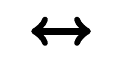
\begin{tikzpicture}[line width=0.6ex]
                        \draw[arrows={<->}]
                        (0,0) -- (5ex,0);
                        \end{tikzpicture}
                }}\!
        }

\newcommand{\lra}{\mpsymbol}
\renewcommand{\mp}{\textrm{mp}}

\newcommand{\fps}[1]{\llangle #1 \rrangle}
\newcommand{\fpsx}{\fps{\bbx}}
\newcommand{\fralg}[1]{\langle #1 \rangle}
\newcommand{\fax}{\fralg{\bbx}}


\newcommand{\plangle}{\moverlay{(\cr<}}
\newcommand{\prangle}{\moverlay{)\cr>}}

\newcommand{\flangle}{\plangle\hphantom{_o}\mathllap{\plangle}}
\newcommand{\frangle}{\mathrlap{\prangle}\hphantom{_o}\prangle}

\newcommand{\skf}[1]{\plangle #1 \prangle}
\newcommand{\fls}[1]{\flangle #1 \frangle}


%\newcommand{\hypj}[1]{J^{\text{hyp}}_{#1}}
\newcommand{\hypj}[1]{J^{\mathbbm{H}}_{#1}}
%\newcommand{\hypj}[1]{\moverlay{\triangle \cr \raisebox{0.025ex}{\scaleobj{0.775}{\times}}   }_{#1}}
%\newcommand{\hypmat}{\moverlay{\triangle \cr \raisebox{0.025ex}{\scaleobj{0.775}{\times}}   }}

%\makeatletter
%\def\moverlay{\mathpalette\mov@rlay}
%\def\mov@rlay#1#2{\leavevmode\vtop{
%                \baselineskip\z@skip \lineskiplimit-\maxdimen
%                \ialign{\hfil$#1##$\hfil\cr#2\crcr}}}
%\makeatother





\newcommand{\meric}{\red \sc}




%\begin Shrug
\newcommand{\shrug}[1][]{%
\begin{tikzpicture}[baseline,x=0.8\ht\strutbox,y=0.8\ht\strutbox,line width=0.125ex,#1]
\def\arm{(-2.5,0.95) to (-2,0.95) (-1.9,1) to (-1.5,0) (-1.35,0) to (-0.8,0)};
\draw \arm;
\draw[xscale=-1] \arm;
\def\headpart{(0.6,0) arc[start angle=-40, end angle=40,x radius=0.6,y radius=0.8]};
\draw \headpart;
\draw[xscale=-1] \headpart;
\def\eye{(-0.075,0.15) .. controls (0.02,0) .. (0.075,-0.15)};
\draw[shift={(-0.3,0.8)}] \eye;
\draw[shift={(0,0.85)}] \eye;
% draw mouth
\draw (-0.1,0.2) to [out=15,in=-100] (0.4,0.95); 
\end{tikzpicture}}
%\end shrug





\showboxdepth=\maxdimen
\showboxbreadth=\maxdimen




\numberwithin{equation}{section}
\setcounter{secnumdepth}{3}



\makeindex

\allowdisplaybreaks

\title{FLOP -- Free List of Open Problems -- \today}




\begin{document}

\begin{center}
	\textbf{\huge{FLOP -- Free List of Open Problems}}
	
	\huge{\today}
\end{center}
\tableofcontents





%############################################################################
%############################################################################
%############################################################################

%					ALGEBRAIC CHAPTER

%############################################################################
%############################################################################
%############################################################################


\chapter{Algebraic Problems}

\section{Algebraic Notation}
\begin{center}
\begin{tabular}{l c l}
	$\C\fralg{x_1,\dots,x_\ttg}$ &  & free $\C$-algebra generated by $x_1,\dots, x_{\ttg}$ \\
	$\C\skf{x_1,\dots,x_\ttg}$ &  & free skew field (nc rationals) of $\C\fralg{x_1,\dots,x_\ttg}$  \\
	$\C\skf{\bbx}_0$ &  & algebra of rationals regular at $0$ \\
	$\C\skf{\bbx \lra \bby}$ &  & universal skew field of fractions of $\C\skf{\bbx}\otimes \C\skf{\bby}$
\end{tabular}
\end{center}



%############################################################################
%############################################################################
%############################################################################


\section{Factoring Invertible Matrices over $\C\fralg{x}\otimes \C\fralg{y}$}
	\label{sec:Elem_Mats}


\begin{problem}
	Suppose $A\in M_n(\C\fralg{\bbx}\otimes \C\fralg{\bby})$. If $A$ is invertible over the $\C$-algebra $\C\fralg{\bbx}\otimes \C\fralg{\bby}$ then do there exist $D,E_1,\dots, E_k\in M_n(\C\fralg{\bbx}\otimes \C\fralg{\bby})$ such that $D$ is diagonal, each $E_i$ is an elementary matrix and $A = DE_1\dots E_k$?
\end{problem}

\begin{remark}
	The above problem is false when $n=2$. Cohn gave the following matrix that is not a product of elementary matrices over $\C[x]\otimes \C[y]$:
	\[
		\bpm 1\otimes 1 + x\otimes y & 1\otimes y^2 \\ -x^2\otimes 1 & 1\otimes 1 - x\otimes y \epm.
	\]
\end{remark}

The above counterexample is nonexistent when our matrices are over $\C\fralg{\bbx}$ instead. The proof of this uses results from \cite{SuslinCohn06}.

\begin{theorem}
	If $A\in M_n(\C\fralg{\bbx})$ is invertible, then there exist $D,E_1,\dots, E_k\in M_n(\C\fralg{\bbx})$ such that $D$ is diagonal, each $E_i$ is an elementary matrix and $A = DE_1\dots E_k$.
\end{theorem}

The Cohn counterexample is essentially the only issue:

\begin{theorem}[Suslin's Stability Theorem]
	Suppose $A\in M_n(\C[t_1,\dots, t_\ttg])$ where $n\geq 3$. If $\det(A) = 1$ then there exist $E_1,\dots, E_k\in M_n(\C[t_1,\dots, t_\ttg])$ such that $A = E_1\dots E_k$.
\end{theorem}

An ``algorithmic" proof of the above theorem can be found in \cite{SuslinPW95}.


\begin{remark}
	An idea related to this is the notion of Jacobian Tame, see \ref{sec:Jac Tame}.
\end{remark}


\begingroup
\renewcommand{\addcontentsline}[3]{}% Remove functionality of \addcontentsline
\renewcommand{\section}[2]{}% Remove functionality of \section

\vspace{1em}

\begin{center}
	{\normalsize \textsc{References}}
\end{center}


\begin{thebibliography}{PW95}

\bibitem[Coh06]{SuslinCohn06}
P.M. Cohn.
\newblock {\em Free Ideal Ring and Localizations in General Rings}.
\newblock Cambridge University Press, 2006.

\bibitem[PW95]{SuslinPW95}
H.J. Park and C.~Woodburn.
\newblock An algorithmic proof of {S}uslin's stability theorem for polynomial
  rings.
\newblock {\em Journal of Algebra}, 178(1):277 -- 298, 1995.

%\bibitem[Swe70]{Swe70}
%Moss~Eisenberg Sweedler.
%\newblock A units theorem applied to hopf algebras and amitsur cohomology.
%\newblock {\em American Journal of Mathematics}, 92(1):259--271, 1970.

\end{thebibliography}


\endgroup






\bigskip



%############################################################################
%############################################################################
%############################################################################


\section{Free L{\"u}roth Theorem}
	\label{sec:Luroth}
\begin{problem}[Free L{\"u}roth Theorem]
Suppose $\k$ is an algebraically closed infinite field and $x_1,\dots, x_g$ are freely noncommuting indeterminates ($g\geq 2$).
If $\k\subsetneq D\subsetneq \k\skf{x_1,\dots, x_\ttg}$ is a subfield, then do there exist $q_1,\dots, q_\tth\in \C\skf{x_1,\dots, x_\ttg}$ 
such that $D = \C\skf{q_1, \dots, q_\tth}$?

In other words, is every non-trivial subfield of $\C\skf{\bbx}$ a free skew field?
\end{problem}


\begin{theorem}[L{\"u}roth's Theorem]

Suppose $\k$ is a field. If $\k \subsetneq D \subsetneq \k(t)$ is a subfield, then there exists $q\in \k(t)$ such that $D = \k(q(t))$.

\end{theorem}

\begin{remark}
	If $\k$ is algebraically closed and infinite, then L{\"u}roth's Theorem holds as well for $\k(t_1,t_2)$.
	
	On the other hand, there are counterexamples to L{\"u}roth's Theorem for $\k(t_1,t_2,t_3)$.
\end{remark}

\begin{remark}
	Schofield \cite{Luroth-Sch85} shows that if $f,g\in \C\skf{\bbx}$, then either $[f,g] = 0$ or $\C\skf{f,g}$ is free.
\end{remark}



\begingroup
\renewcommand{\addcontentsline}[3]{}% Remove functionality of \addcontentsline
\renewcommand{\section}[2]{}% Remove functionality of \section

\vspace{1em}

\begin{center}
	{\normalsize \textsc{References}}
\end{center}


\begin{thebibliography}{Sch85}

\bibitem[Sch85]{Luroth-Sch85}
Schofield, A. H.
\newblock Representations of rings over skew fields.
\newblock {\em London Mathematical Society Lecture Note Series}, 1985.
\end{thebibliography}


\endgroup


\bigskip


%############################################################################
%############################################################################
%############################################################################



\section{Free Bertini Theorem - \textit{SOLVED!}}
	\label{sec:FreeBertini}
	

\noindent Great result solved in \cite{Vol19}


We say $f\in \bbk\fralg{\bbx}$ \textbf{factors} if $f = f_1f_2$ for some nonconstant $f_1,f_2\in \bbk\fralg{\bbx}$. Otherwise $f$ is \textbf{irreducible} over $\bbk$.
A nonconstant $f\in \bbk\fralg{\bbx}$ is \textbf{composite} if there exist $h\in \bbk\fralg{\bbx}$ and a univariate polynomial $p\in \bbk[t]$ such that $\deg(p)>1$ and $f = p\circ h = p(h)$.


\begin{theorem}
	If $f\in \bbk\fralg{\bbx}\setminus \bbk$ is not composite, then $f - \lambda$ is irreducible over $\overline{\bbk}$ for all but finitely many $\lambda\in\overline{\bbk}$.
\end{theorem}









%############################################################################
%############################################################################
%############################################################################


\section{Rational Bertini Theorem}
	\label{sec:RatBertini}
	

A nonconstant $f\in \bbk\skf{\bbx}$ is \textbf{composite} if there exist $h\in \bbk\skf{\bbx}$ and a univariate rational $p\in \bbk(t)$ such that $p$ is not linear or inverse linear and $f = p\circ h = p(h)$.





%############################################################################
%############################################################################
%############################################################################


\section{Jacobian Tame}
	\label{sec:Jac Tame}

An automorphism $\tau$ of the free algebra $\C\fralg{x_1,\dots, x_\ttg}$ is {\bf elementary} if $\tau:x_i \mapsto x_i$ 
	for $i\neq j$ and $\tau:x_j \mapsto cx_j + f$, where $c\in \C$ and $f\in \C\fralg{x_1,\dots, x_{j-1}, x_{j+1},\dots, x_\ttg}$.
We say an automorphism is {\bf tame} if it is a composition of elementary automorphisms.
If the automorphism is not tame, then it is {\bf wild}.

In \cite{U07} it is shown that the Anick automorphism, 
\[
	\delta(x,y,z) = (x + z(xz - zy), y + (xz - zy)z, z)\in \C\fralg{x,y,z}
\]
is wild.
Looking at it, the Anick automorphism doesn't seem particularly ``wild," so maybe this can be improved?
Perhaps it is something about Jacobian matrices?

\begin{definition}
	We say an automorphism $\tau$ of $\C\fralg{x_1,\dots, x_\ttg}$ is \textbf{Jacobian Tame} if
	$J_\tau = DE_1\dots E_k$, where $D\in M_\ttg(\C\fralg{\bbx'}^{opp}\otimes \C\fralg{\bbx})$ is diagonal and
	$E_1,\dots, E_k\in M_\ttg(\C\fralg{\bbx'}^{opp}\otimes \C\fralg{\bbx})$ are elementary matrices.
	
	If such a factorization does not exist, then we say $\tau$ is \textbf{Jacobian wild}.
\end{definition}


\begin{problem}
	Are there any Jacobian wild automorphisms of the free algebra?
	The only known (to me) example of a wild automorphism of $\C\fralg{x,y,z}$ is Jacobian tame (this is explained below).
	
	In the commutative case there are no Jacobian wild automorphisms.
	Every automorphism of $\C[t_1,t_2]$ is tame, hence Jacobian tame.
	If $\phi$ is an automorphism of $\C[t_1,\dots, t_\ttg]$ with $\ttg>2$, then its Jacobian matrix
	$J_\phi\in M_\ttg(\C[t_1,\dots, t_\ttg,t_1',\dots,t_\ttg'])$ factors into such a product by Suslin's Stability Theorem (see \ref{sec:Elem_Mats}), thus is Jacobian tame.
\end{problem}

I will be using the transposed Jacobian matrix: $J_\tau \in M_\ttg(\C\fralg{\bbx'}^{opp}\otimes \C\fralg{\bbx})$ where the $i^\text{th}$ column of $J_\tau$ corresponds to the derivatives of $\tau_i$.

It turns out that the Anick automorphism 
\[
	\delta(x,y,z) = (x + z(xz - zy), y + (xz - zy)z, z)\in \C\fralg{x,y,z}
\]
has a Jacobian matrix that can be written as a product of elementary matrices.
The Jacobian matrix of $\delta$ is
\[
	J_\delta = 
	\bpm
		1\otimes 1 + z'\otimes z & 1\otimes z^2 & 0 \\
		-(z')^2\otimes 1 & 1 - z'\otimes z & 0 \\
		\zeta_1 & \zeta_2 & 1
	\epm
\]
where $\zeta_1 = 1\otimes xz+ x'z'\otimes 1 - 1\otimes zy - z'\otimes y$ and 
	$\zeta_2 = x\otimes z + z'x'\otimes 1 - 1\otimes yz - y'z'\otimes 1$.
Let $E_{i,j}(\alpha) = I + \alpha e_{i,j}$ ($e_{i,j}$ has a $1$ in the $i,j$ entry and 0's elsewhere) and observe
\[
	J_\delta E_{3,1}(-\zeta_1)E_{3,2}(-\zeta_2) = 
	\bpm
		1\otimes 1 + z'\otimes z & 1\otimes z^2 & 0 \\
		-(z')^2\otimes 1 & 1 - z'\otimes z & 0 \\
		0 & 0 & 1
	\epm.
\]
In 1966, Cohn proved that
\[
	\mathfrak{C} = 
	\bpm
		1\otimes 1 + z'\otimes z & 1\otimes z^2\\
		-(z')^2\otimes 1 & 1 - z'\otimes z
	\epm
\]
cannot be written as a product of elementary matrices over $\mathbb{F}[z'\otimes 1,1\otimes z]$.
This is a crucial aspect of Umirbaev's (\cite{U07}) proof that the Anick automorphism is wild.
However, Park and Woodburn \cite{PW95} give a decomposition of $(\begin{smallmatrix} \mathfrak{C} & 0 \\ 0 & 1 \end{smallmatrix})$ 
	into a product of elementary matrices:
\begin{align*}
	J_\delta &E_{3,1}(-\zeta_1)E_{3,2}(-\zeta_2) =
	\bpm
		1\otimes 1 + z'\otimes z & 1\otimes z^2 & 0 \\
		-(z')^2\otimes 1 & 1 - z'\otimes z & 0 \\
		0 & 0 & 1
	\epm\\
	= &	
	E_{2,3}(-z'\otimes 1)E_{1,3}(1\otimes z)E_{3,2}(1\otimes z)E_{3,1}(z'\otimes 1)\\
	& E_{2,3}(z'\otimes 1)E_{1,3}(-1\otimes z)E_{3,2}(-1\otimes z)E_{3,1}(-z'\otimes 1).
\end{align*}
Thus
\begin{align*}
	J_\delta = & E_{2,3}(-z'\otimes 1)E_{1,3}(1\otimes z)E_{3,2}(1\otimes z)E_{3,1}(z'\otimes 1)\\
	&E_{2,3}(z'\otimes 1)E_{1,3}(-1\otimes z)E_{3,2}(-1\otimes z)E_{3,1}(-z'\otimes 1)E_{3,2}(\zeta_2)E_{3,1}(\zeta_1).
\end{align*}
Thus, the Jacobian matrix of $\delta$ factors as a product of elementary matrices even though it is wild.


\vspace{1em}



Naturally, a positive answer to the Problem in \ref{sec:Elem_Mats} would show that every automorphism is Jacobian Tame.
On the other hand, a negative answer to the Problem in \ref{sec:Elem_Mats} would only serve to complicate things since a Jacobian matrix will certainly look quite different from a generic matrix in $\GL_\ttg(\C\fralg{\bbx'}^{opp}\otimes \C\fralg{\bbx})$.



%\begingroup
%\renewcommand{\addcontentsline}[3]{}% Remove functionality of \addcontentsline
%\renewcommand{\section}[2]{}% Remove functionality of \section
%
%\vspace{1em}
%
%\begin{center}
%	{\normalsize \textsc{References}}
%\end{center}
%
%
%\begin{thebibliography}{Umi07}
%
%\bibitem[PW95]{PW95}
%H.J. Park and C.~Woodburn.
%\newblock An algorithmic proof of {S}uslin's stability theorem for polynomial
%  rings.
%\newblock {\em Journal of Algebra}, 178(1):277 -- 298, 1995.
%
%\bibitem[Umi07]{U07}
%U.~U. Umirbaev.
%\newblock The {A}nick automorphism of free associative algebras.
%\newblock {\em J. Reine Angew. Math.}, 605:165--178, 2007.
%
%\end{thebibliography}
%
%
%\endgroup







\bigskip

%############################################################################
%############################################################################
%############################################################################

\section{Tensor Product of Free Skew Fields}
	\label{sec:TPFSF}


\begin{problem}
	Classify the invertible elements of $\C\skf{\bbx}\otimes \C\skf{\bby}$.
	The expectation is that if $Q$ and $Q^{-1}$ are in $\C\skf{\bbx}\otimes \C\skf{\bby}$, then $Q = r\otimes s$, for some nonzero elements $r\in \C\skf{\bbx}$ and $s\in \C\skf{\bby}$.
\end{problem}

The following was proven in \cite{Swe70} using techniques that seemingly don't translate well to the noncommutative setting.

\begin{theorem}
	Suppose $A$ and $B$ are commutative domains over an algebraically closed field $\k$ and $\k$ is algebraically closed in $A$ and $B$. If $z\in A\otimes B$ is invertible, then $z = a\otimes b$ for some invertible elements $a\in A$ and $b\in B$.
\end{theorem}

The following two simplifications have been proven using Complex Analysis and Realization Theory:

\begin{proposition}
	Suppose $r\in \C\skf{\bbx}$ and $s\in \C\skf{\bby}$.
	If $(1\otimes 1 - r\otimes s)^{-1}\in \C\skf{\bbx}\otimes \C\skf{\bby}$ then either $r$ or $s$ is constant.
	
	Suppose $\ttg\geq k$ and $r_1,\dots, r_k\in \C\skf{\bbx}$. If $(1\otimes 1 - \sum_{i=1}^k r_i\otimes y_i)^{-1}\in \C\skf{\bbx}\otimes \C\skf{\bby}$ then $r_1,\dots, r_k$ are all constant.
\end{proposition}


Although this is progress, in general an element of $\C\skf{\bbx\lra \bby}$ will not have inversion height $1$.
So additional ideas or techniques must be developed to answer the other cases.

The tensor product membership problem is strongly related to the rational automorphism problem as well, although that may require an understanding of domains.





\begingroup
\renewcommand{\addcontentsline}[3]{}% Remove functionality of \addcontentsline
\renewcommand{\section}[2]{}% Remove functionality of \section

\vspace{1em}

\begin{center}
	{\normalsize \textsc{References}}
\end{center}


\begin{thebibliography}{Swe70}

%\bibitem[Coh06]{Cohn06}
%P.M. Cohn.
%\newblock {\em Free Ideal Ring and Localizations in General Rings}.
%\newblock Cambridge University Press, 2006.
%
%\bibitem[PW95]{PW95}
%H.J. Park and C.~Woodburn.
%\newblock An algorithmic proof of {S}uslin's stability theorem for polynomial
%  rings.
%\newblock {\em Journal of Algebra}, 178(1):277 -- 298, 1995.

\bibitem[Swe70]{Swe70}
Moss~Eisenberg Sweedler.
\newblock A units theorem applied to hopf algebras and amitsur cohomology.
\newblock {\em American Journal of Mathematics}, 92(1):259--271, 1970.

\end{thebibliography}


\endgroup


%############################################################################
%############################################################################
%############################################################################


\bigskip

\section{Rational Automorphisms}
	\label{sec:RatAuts}


\begin{problem}
	Suppose $\bbr\in (\C\skf{x_1,\dots, x_\ttg})^\ttg$. Find an evaluation criterion that is necessary and sufficient for the induced map $\rho:\C\skf{x_1,\dots, x_\ttg}\to\C\skf{x_1,\dots, x_\ttg}$ ($\rho(x_i) = \bbr_i$) to be an automorphism.
\end{problem}

An evaluation criterion is some condition on $\bbr$ when we treat it as a function.
For example, injective, surjective, etc.

\begin{conjecture}
	Suppose $\bbr\in (\C\skf{x_1,\dots, x_\ttg})^\ttg$.
	The following are equivalent:
	\begin{enumerate}
		\item there exists a free, Euclidean open and Euclidean dense set $\Omega$ such that $\bbr\lvert_\Omega$ is injective;
		\item $J_\bbr$ is an invertible element of $M_\ttg(\C\skf{\bbx'}^{opp}\otimes \C\skf{\bbx})$;
		\item the induced map $\rho:\C\skf{\bbx}\to \C\skf{\bbx}$ given by $\rho(x_i) = \bbr_i$ is an automorphism.
	\end{enumerate}
\end{conjecture}


This is simply a best guess conjecture at the moment. Clearly, $(3)\Rightarrow (1),(2)$.
Condition $(1)$ is seemingly strange, but the na{\"i}ve attempt of requiring injective on its domain is insufficient.

\begin{example}
	Let $\bbr(x,y) = (x, y - x^2y)$.
	This induces a rational automorphism, however $\bbr(1,\alpha) = \bbr(1,\beta)$, hence $\bbr$ is not injective on its domain (in fact, the points where it is not injective are exactly the points where $\bbr^{-1}$ is not defined).
	If $\Omega = \set{(X,Y)\in M_n(\C)^2 \, : \, \det(I_n - X^2)\neq 0}$, then $\Omega$ is free, Euclidean open and dense and $\bbr$ is injective on $\Omega$.
\end{example}

Let us see a slightly harder example.

\begin{example}
	Let $\bbr(x,y) = (x, y - xyx)$.
	Naturally $\bbr$ is not injective on $\C^2$ since $\bbr(1,\alpha) = \bbr(1,\beta)$.
	However, $\bbr$ does not induce a rational automorphism and this fact is a bit harder to see.
	
	The first observed reason why is found by using formal power series.
	Since the derivative of $\bbr$ is invertible on some free neighborhood of $0$, it must have a local inverse that we can find as a power series.
	It turns out that
	\[
		f(x,y) = (x, \sum_{n=0}^\infty x^nyx^n)
	\]
	is the formal power series representation of $\bbr^{-1}$.
	If one tries to write down a realization for $f$, then a contradiction is eventually attained showing that $f$ is not a rational power series.
	Thus, $\bbr$ does not induce a rational automorphism.
	This doesn't give us too much information at the moment, since it reveals little about the injectivity of $\bbr$.
	
	Our alternative approach is to use the idea behind the conception of hyporationals: the matrix identity $\vecc(AXB) = \vecc(X)(A^T\otimes B)$.
	Let $f = (\bbr^{-1})_2$.
	Since $f(x,y)$ is satisfies the equation $f(x,y) = y + xf(x,y)x$, we evaluate on a pair of matrices $(X,Y)$ (when it makes sense) and note we have
	\[
		f(X,Y) = Y + Xf(X,Y)X.
	\]
	Taking the vectorization of both sides and rearranging, we have
	\[
		\vecc(f(X,Y))(I_n\otimes I_n - X^T\otimes X) = \vecc(I_n)(I_n\otimes Y).
	\]
	Multiplying on the right by an inverse we see
	\[
		\vecc(f(X,Y)) = \vecc(I_n)(I_n\otimes Y)\left(I_n\otimes I_n - X^T\otimes X\right)^{-1}.
	\]
	Thus, for any matrix $X$ where $(I_n\otimes I_n - X^T\otimes X)$ is invertible we have $(X,Y)$ is in the domain of $\bbr^{-1}$.
	As pointed out in \ref{sec:TPFSF}, the function $(1\otimes 1-x'\otimes x)^{-1}\notin \C\skf{x'}\otimes \C\skf{x}$.
	However, a consequence of its (first) proof is that there is no free Euclidean open and Euclidean dense set upon which $(1\otimes 1-x'\otimes x)$ is invertible.
	Thus, $\bbr$ fails to satisfy requirement $(1)$ from the Conjecture and $\bbr$ does not induce a rational automorphism.
	
	To see why $q = (1\otimes 1-x'\otimes x)$ fails to be injective on a ``big" set, suppose $\Omega$ is any nonempty free open set upon which $q$ is invertible.
	If $\lambda$ and $\mu$ are any eigenvalues of $X$ then $\lambda\mu$ is an eigenvalue of $X^T\otimes X$ and $1-\lambda\mu$ is an eigenvalue of $q(X^T,X)$.
	Hence, if $X\in \Omega$, then for each eigenvalue $\lambda$ of $X$, $\lambda^{-1}$ is not an eigenvalue of any matrix in $\Omega$.
	Thus, the eigenvalues of $q(X^T,X)$, taken over all $X\in \Omega$ partition the complex plane.
	However, since $\Omega$ is an open set, the eigenvalues of $q$ must contain open sets.
	Thus, the eigenvalues of $q$ must miss an open set of $\C$, therefore $\Omega$ cannot be dense since a nonconstant element of $\C\skf{x'}\otimes \C\skf{x}$ must have dense eigenvalues on a dense set.
\end{example}





%\begingroup
%\renewcommand{\addcontentsline}[3]{}% Remove functionality of \addcontentsline
%\renewcommand{\section}[2]{}% Remove functionality of \section
%
%\vspace{1em}
%
%\begin{center}
%	{\normalsize \textsc{References}}
%\end{center}
%
%
%\begin{thebibliography}{Swe70}
%
%%\bibitem[Coh06]{Cohn06}
%%P.M. Cohn.
%%\newblock {\em Free Ideal Ring and Localizations in General Rings}.
%%\newblock Cambridge University Press, 2006.
%%
%%\bibitem[PW95]{PW95}
%%H.J. Park and C.~Woodburn.
%%\newblock An algorithmic proof of {S}uslin's stability theorem for polynomial
%%  rings.
%%\newblock {\em Journal of Algebra}, 178(1):277 -- 298, 1995.
%
%\bibitem[Swe70]{Swe70}
%Moss~Eisenberg Sweedler.
%\newblock A units theorem applied to hopf algebras and amitsur cohomology.
%\newblock {\em American Journal of Mathematics}, 92(1):259--271, 1970.
%
%\end{thebibliography}
%
%
%\endgroup


%############################################################################
%############################################################################
%############################################################################




\bigskip

\section{Rational Derivatives - \textit{SOLVED!}}
	\label{sec:RatDeriv}
	
\textit{
Originally posed by James Pascoe to Meric Augat in March of 2020.
}

\vspace{1em}

Let $\bbx = \set{x_1,\dots, x_\ttg}$ and $\bbh = \set{h_1,\dots, h_\ttg}$ be a sets of freely noncommuting indeterminates.
Let $\C\fpsx$ denote the formal power series in $\bbx$ and let $\C\skf{\bbx}_0$ denote the rational formal power series.
If $S\in \C\fpsx$ and $w$ is a word, then $[S,w]$ is the coefficient of $w$ appearing in $S$.
For any word $w$ and series $S\in \C\fpsx$, we let $w^{-1}S = \sum_{v\in \fax} [S,wv]v$.


\begin{proposition}
	Suppose $f\in \C\fpsx$.
	If $Df(\x)[\h] \in \C\skf{\bbx,\bbh}_0$ then $f\in \C\skf{\bbx}_0$.
\end{proposition}

\begin{proof}
	For each $1\leq i\leq \ttg$ we let $\partial_i f := Df(\x)[0,\dots,0,h_i,0,\dots,0]$ and note $\partial_i f\in \C\skf{\bbx,\bbh}_0$.
	Next, we write
	\[
		f = c_0 + \sum_{i=1}^\ttg x_i f_i
	\]
	where each $f_i\in \C\fpsx$.
	Hence,
	\[
		\partial_i f = h_if_i + \sum_{j=1}^\ttg x_j \partial_i f_j\in \C\skf{\bbx,\bbh}_0
	\]
	and it follows that $h_i^{-1}\partial_if_i = f_i\in \C\skf{\bbx,\bbh}_0$ since $\partial_i f_i$ is contained in a stable submodule.
	Therefore, $f = c_0 + \sum_{i=1}^\ttg x_i f_i\in \C\skf{\bbx}_0$ since each $f_i$ is rational.
\end{proof}


The argument below shows it for generalized series. Notation and ideas are pulled from \cite{RatDeriv-Vol18}.
Notably, if $v$ is a word, $L_v S = \sum_{w\in \fax} [S,vw]$.

\begin{remark}
	Let $\cA = M_n(\C)$ for some $n$.
	If $f\in \cA\fpsx$ then
	\[
		f = f_0 + \sum_{i=1}^\ttg L_{x_i} f
	\]
	and
	\[
		Df(\x)[\h] = \sum_{i=1}^\ttg L_{h_i}Df(\x)[\h] + \sum_{i=1}^\ttg L_{x_i}Df(\x)[\h].
	\]
	If $f_i(\x,h_i) = L_{h_i}Df(\x)[\h]$, then $f_i(\x,x_i) = L_{x_i}f$.
	Hence, if $Df(\x)[\h]$ is rational, then so is $L_{h_i}Df(\x)[\h]$ and consequently so is $L_{x_i}f$.
	Therefore, $f$ is rational since it is a sum of rational series.	
\end{remark}








\begingroup
\renewcommand{\addcontentsline}[3]{}% Remove functionality of \addcontentsline
\renewcommand{\section}[2]{}% Remove functionality of \section

\vspace{1em}

\begin{center}
	{\normalsize \textsc{References}}
\end{center}


\begin{thebibliography}{Vol18}

\bibitem[Vol18]{RatDeriv-Vol18}
Jurij Vol{\v c}i{\v c}.
\newblock Matrix coefficient realization theory of noncommutative rational functions.
\newblock {\em Journal of Algebra}, 499: 397 - 437, 2018.
\end{thebibliography}


\endgroup













\section{Artin approximation theorem}
	\label{sec:ArtinApprox}
	





\begin{problem}
	Suppose $\bbk\fpsx$ is the algebra of formal power series with freely noncommuting indeterminates $\bbx = \set{x_1,\dots, x_\ttg}$ over the field $\bbk$.
	Suppose $\bby = \set{y_1,\dots, y_\tth}$ is a distinct set of freely noncommuting indeterminates and let 
	\[
		f(\x,\y) = 0
	\]
	be a system of polynomial equations in $\bbk\fralg{\bbx,\bby}$, and let $c$ be a positive integer.
	Then given a formal power series solution $\hat{\y}(\x)\in \bbk\fpsx$, there is an algebraic solution $\y(\x)$ consisting of algebraic power series such that
	\[
		\hat{\y}(\x) \equiv \y(\x) \mod (\x)^c
	\]
\end{problem}


In the classical setting, this problem uses the Implicit function theorem and some refinements of the IFT.








\vspace{1em}


Max pencil kernels and Makar-Limanov

Nc Noether Problem.

Artin-Schreier



\chapter{Convexity Problems}

\begin{itemize}
\item What sets spectradrops apart from general matrix convex sets?

\item Positivstellensatz for spectradrops

\item Including a drop into the matrix cube, or other spectrahedron. A variation
of asking about approximating above by a specrahedron.

\end{itemize}

\chapter{Geometry}

Polynomial automorphisms between free loci.


\chapter{Analysis}

\begin{itemize}
	\item Local Operator Monotonicity vs. Global Operator Monotonicity
	
	\item Jerk functions and their realizations
	
	\item Weierstrass preparation theorem
	
	\item NC rational function defined on $\B(\cH)$

\end{itemize}







\begin{thebibliography}{6}

\bibitem[Coh06]{Cohn06}
P.M. Cohn.
\newblock {\em Free Ideal Ring and Localizations in General Rings}.
\newblock Cambridge University Press, 2006.


\bibitem[PW95]{PW95}
H.J. Park and C.~Woodburn.
\newblock An algorithmic proof of {S}uslin's stability theorem for polynomial
  rings.
\newblock {\em Journal of Algebra}, 178(1):277 -- 298, 1995.

\bibitem[Umi07]{U07}
U.~U. Umirbaev.
\newblock The {A}nick automorphism of free associative algebras.
\newblock {\em J. Reine Angew. Math.}, 605:165--178, 2007.


\bibitem[Sch85]{Sch85}
Schofield, A. H.
\newblock Representations of rings over skew fields.
\newblock {\em London Mathematical Society Lecture Note Series}, 1985.


\bibitem[Swe70]{Swe70}
Moss~Eisenberg Sweedler.
\newblock A units theorem applied to {H}opf algebras and {A}mitsur cohomology.
\newblock {\em American Journal of Mathematics}, 92(1):259--271, 1970.



\bibitem[Vol18]{Vol18}
Jurij Vol{\v c}i{\v c}.
\newblock Matrix coefficient realization theory of noncommutative rational functions.
\newblock {\em Journal of Algebra}, 499: 397 - 437, 2018.

\bibitem[Vol19]{Vol19}
Jurij Vol{\v c}i{\v c}.
\newblock Free Bertini's Theorem and applications.
\newblock \url{https://arxiv.org/pdf/1908.08948.pdf}.


\end{thebibliography}











\end{document}











